\documentclass{article}
\hbadness=10000

% ---- Font package (research paper style) ----
\usepackage{newtxtext,newtxmath} % Times-like professional font

\usepackage[utf8]{inputenc}
\usepackage[T1]{fontenc}
\usepackage{amsmath}
\usepackage{xcolor} % Add this package for \textcolor
\usepackage{fancyhdr} % Add this package
\usepackage{ulem} % Add this package for better underlining
\usepackage{graphicx} % Add this package for including images
\usepackage{hyperref}
\usepackage{listingsutf8}  % instead of just listings
\usepackage{listingsutf8} % UTF-8 capable listings
\lstset{
    breaklines=true,               % Enable line breaking
    inputencoding=utf8,            % Set UTF-8 input encoding
    keywordstyle=\color{blue}\bfseries,
    commentstyle=\color{green!50!black},
    stringstyle=\color{orange},
    backgroundcolor=\color{gray!10},
    frame=single
}

\hypersetup{
    colorlinks=true,
    linkcolor=blue,
    citecolor=blue,
    filecolor=blue,
    urlcolor=blue,
    pdfborder={0 0 0}
}

\title{\LARGE\bfseries Comprehensive Data Science Documentation}
\author{
    \textbf{Prosenjit Mondol} \\
    \normalsize Data Scientist \\ 
    \normalsize \href{mailto:prosenjit1156@email.com}{prosenjit1156@email.com}
}
\date{\today}

\pagestyle{fancy} % Enable fancy header
\fancyhead[L]{My Personal Documentations} % Left side header with documentation name
\fancyhead[C]{} % Center header empty
\fancyhead[R]{Prosenjit} % Right side header empty
\renewcommand{\headrulewidth}{1pt} % Add a horizontal line under the header

\begin{document}

\maketitle

\tableofcontents % <-- Add this line for list view

\newpage % Start a new page after the table of contents

\section{Data Preprocessing}
\begin{itemize}
    \item \textbf{\textcolor{blue}{\dotuline{Sampling}}}\\
        Sampling techniques are used to select a representative subset of data from a large population to reduce the computational complexity and improve the efficiency of the analysis.
    \item \textbf{\textcolor{blue}{\dotuline{Transformation}}}\\
    Transformation techniques involve manipulating raw data to create a single input, such as scaling, normalization, or encoding categorical data.
    \item \textbf{\textcolor{blue}{\dotuline{Denoising}}}\\
    Denoising techniques remove unwanted noise from the data that can lead to inaccurate results.
    \item \textbf{\textcolor{blue}{\dotuline{Imputation}}}\\
    Imputation techniques are used to fill in missing values in the data using statistical methods.
    \item \textbf{\textcolor{blue}{\dotuline{Feature extraction}}}\\
    Feature extraction techniques help to identify and extract relevant features from the data that are significant in a particular context.
    \item \textbf{\textcolor{blue}{\dotuline{Normalization}}}\\
    Normalization techniques are used to organize data for more efficient access and processing.

\end{itemize}


\section{Handle Categorical Data}

Categorical data is a type of data that represents qualitative or nominal characteristics, such as gender, occupation, Categorical data cannot be measured or compared using mathematical operations like addition or subtraction.
\subsection{Different Encoding Methods for Categorical Data}
\begin{itemize}
    \item \textbf{\textcolor{blue}{\dotuline{One-Hot Encoding}}}\\
    One-Hot Encoding creates a new binary column for each category.
    \begin{lstlisting}[language=Python, caption={Logistic Regression Example}, label={lst:logreg}, backgroundcolor=\color{gray!10}, frame=single, keywordstyle=\color{blue}\bfseries, commentstyle=\color{green!50!black}, stringstyle=\color{orange}]
X = pd.get_dummies(X)
print(X)
    \end{lstlisting}
    \item \textbf{\textcolor{blue}{\dotuline{Label Encoding}}}\\
    Label Encoding assigns a numerical value to each category.
    \begin{center}
        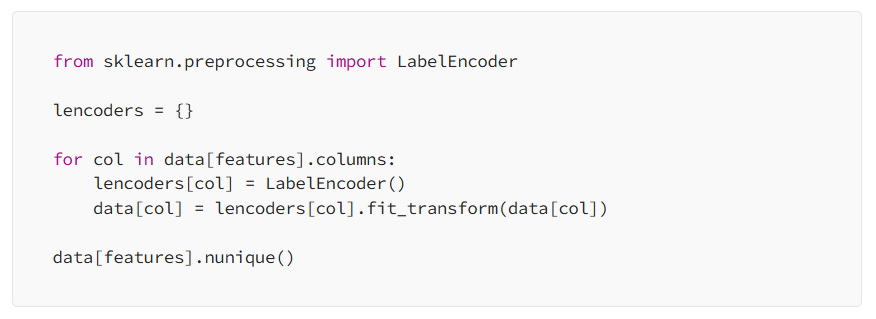
\includegraphics[width=0.5\textwidth]{label encoding} % Replace 'example-image' with your image filename (without extension)
    \end{center}
    \item \textbf{\textcolor{blue}{\dotuline{Binary Encoding}}}\\
    Binary Encoding creates new columns representing each category.
\end{itemize}

\subsection{Looking at null or missing values}
\begin{itemize}
    \item \textbf{\textcolor{blue}{\dotuline{Mean Imputation}}}\\
    Mean imputation is a simple and widely used method for filling in missing values. 
    \item \textbf{\textcolor{blue}{\dotuline{Mode Imputation}}}\\
    Mode imputation is a method for filling in missing values that is similar to mean imputation, but instead of using the mean, it uses the mode of the available values in a column.
    \item \textbf{\textcolor{blue}{\dotuline{K-Nearest Neighbor (KNN) Imputation}}}\\
    KNN imputation is a method for filling in missing values that is based on the distance between data poionts.
    \begin{center}
    \begin{lstlisting}[language=Python, caption={Logistic Regression Example}, label={lst:logreg}, backgroundcolor=\color{gray!10}, frame=single, keywordstyle=\color{blue}\bfseries, commentstyle=\color{green!50!black}, stringstyle=\color{orange}]
    # Multiple Imputation by Chained Equations
    from sklearn.experimental import enable_iterative_imputer
    from sklearn.impute import IterativeImputer

    #mputed_data = df[numerical_columns].copy(deep=True) 
    mice_imputer = IterativeImputer()
    data[numerical_columns] = mice_imputer.fit_transform(data[numerical_columns])
    \end{lstlisting}
    \end{center}
\end{itemize}

\section{Checking imblanced in target variable}
\begin{itemize}
    \item \textbf{\textcolor{blue}{\dotuline{Handling imbalanced data using oversampling}}}\\
    oversampling is a method for handling imbalanced data by increasing the size of the minority class.
    \begin{center}
    \begin{lstlisting}[language=Python, caption={Logistic Regression Example}, label={lst:logreg}, backgroundcolor=\color{gray!10}, frame=single, keywordstyle=\color{blue}\bfseries, commentstyle=\color{green!50!black}, stringstyle=\color{orange}]
from sklearn.utils import resample

no = normalized_data[normalized_data.RainTomorrow == 0]
yes = normalized_data[normalized_data.RainTomorrow == 1]
yes_oversampled = resample(yes, replace=True, n_samples=len(no), random_state=123)
oversampled_data = pd.concat([no, yes_oversampled])

fig = plt.figure(figsize = (8,5))
sns.countplot(x='RainTomorrow', data = oversampled_data, palette = "Set1").set(title='RainTomorrow Indicator No(0) and Yes(1) after Oversampling (Balanced Dataset)')
    \end{lstlisting}
    \end{center}
    
    \item \textbf{\textcolor{blue}{\dotuline{How multicollinearity affects decision trees}}}\\
    Multicollinearity affects decision trees by reducing the importance and accuracy of the input features.
    \begin{center}
    \begin{lstlisting}[language=Python, caption={Logistic Regression Example}, label={lst:logreg}, backgroundcolor=\color{gray!10}, frame=single, keywordstyle=\color{blue}\bfseries, commentstyle=\color{green!50!black}, stringstyle=\color{orange}]
    #the heat map of the correlation
    plt.figure(figsize=(16,10))
    sns.heatmap(X.corr(), annot=True, cmap='RdYlGn')
    \end{lstlisting}
    \end{center}
\end{itemize}

\section{Outliner Detection}
\begin{itemize}
    \item \textbf{\textcolor{blue}{\dotuline{Boxplot Method}}}\\
    One of the simplest and most popular methods for detecting outliers is the box-plot.
    \begin{center}
    \begin{lstlisting}[language=Python, caption={Logistic Regression Example}, label={lst:logreg}, backgroundcolor=\color{gray!10}, frame=single, keywordstyle=\color{blue}\bfseries, commentstyle=\color{green!50!black}, stringstyle=\color{orange}]
        plt.figure(figsize=(50,25))
        sns.boxplot(data=scaled_data[numerical_features])
    \end{lstlisting}
    \end{center}
    \newpage

    \item \textbf{\textcolor{blue}{\dotuline{Z-Score Method}}}\\
    The Z-Score method is a simple and widely used method for detecting outliers.
    \begin{center}
        \begin{lstlisting}[language=Python, caption={Logistic Regression Example}, label={lst:logreg}, backgroundcolor=\color{gray!10}, frame=single, keywordstyle=\color{blue}\bfseries, commentstyle=\color{green!50!black}, stringstyle=\color{orange}]
from scipy import stats
import numpy as np

# Calculate Z-scores for each value in the numerical features
z_scores = np.abs(stats.zscore(scaled_data[numerical_features]))

# Identify outliers (e.g., Z-score > 3)
outliers = (z_scores > 3)

# Print rows with outliers
print(scaled_data[outliers.any(axis=1)])
\end{lstlisting}
\end{center}
 \item \textbf{\textcolor{blue}{\dotuline{Transformation}}}\\
 Transformation involves transforming the data to a different scale to reduce the impact of the outliers.   
 \begin{center}
    \begin{lstlisting}[language=Python, caption={Logistic Regression Example}, label={lst:logreg}, backgroundcolor=\color{gray!10}, frame=single, keywordstyle=\color{blue}\bfseries, commentstyle=\color{green!50!black}, stringstyle=\color{orange}]
        from sklearn.preprocessing import PowerTransformer
        # Apply Power Transformation to the numerical features  
        power_transformer = PowerTransformer()
        scaled_data[numerical_features] = power_transformer.fit_transform(scaled_data[numerical_features])    
    \end{lstlisting}    
    \end{center}
\end{itemize}
\newpage


\section{Let’s see how it fared in prediction using Logistic Regression}
\begin{center}
\begin{lstlisting}[language=Python, caption={Logistic Regression Example}, label={lst:logreg}, backgroundcolor=\color{gray!10}, frame=single, keywordstyle=\color{blue}\bfseries, commentstyle=\color{green!50!black}, stringstyle=\color{orange}]
# Train a logistic regression model on the training set
from sklearn.metrics import accuracy_score
from sklearn.linear_model import LogisticRegression

# Instantiate the model
logreg = LogisticRegression(solver='liblinear', random_state=0)

# Fit the model
logreg.fit(X_train, y_train)

# Predict on the test set
y_pred_test = logreg.predict(X_test)

print('Model accuracy score: {0:0.4f}'.format(accuracy_score(y_test, y_pred_test)))
\end{lstlisting}
\end{center}
\vspace{1cm} % adjust cm as needed


\section{Algorithms}
\subsection{Simple Linear Regression}
The output is shown in the best fit line.
\begin{align*}
    y &= mx + C \\
    h_0(x) &= \theta_0 + \theta_1 x \\
    h_0(x) &= \hat{y}  \quad \text{(predicted value)} \\
    error= y - \hat{y} \\
\end{align*}
Here, $\theta_0$ is the intercept, $\theta_1$ is the slope or cofficient.\\
if $x=0$, then $h_0(x) = \theta_0$ (intercept).\\

\begin{figure}[h!]
    \centering
    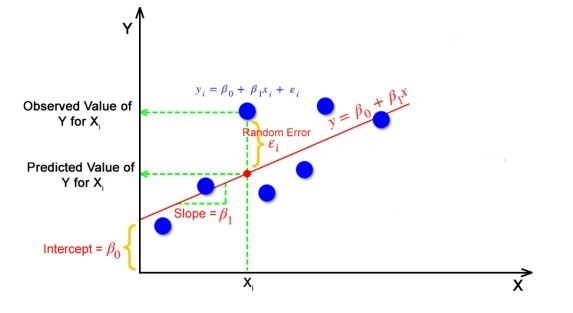
\includegraphics[width=0.7\textwidth]{best_fit.png} % Ensure this file exists in your folder
    \caption{Simple Linear Regression: Best Fit Line, Intercept, Slope, and Error}
    \label{fig:linear_regression}
\end{figure}
\vspace{1cm} % adjust cm as needed

\subsection{Convergence Algorithm \textit{(Optimize the changes of theta\_1 values)}}
Repeat until convergence:
\begin{align*}  
    \theta_j &= \theta_j - \alpha \cdot \frac{\partial J(\theta_j)}{\partial \theta_j} 
\end{align*}

\section{Handle missing values}
why it not

\newpage


\section{Models}

\subsection{Convolutional Neural Networks (CNNs)}
\noindent
\begin{center}  
    \fcolorbox{blue}{blue!10}{
        \parbox{0.95\linewidth}{
            \textbf{Definition:} \\
            Convolutional Neural Networks (CNNs) are deep learning models designed for image analysis, using convolutional layers to automatically extract hierarchical spatial features, pooling layers to reduce dimensionality, and fully connected layers for classification or prediction.
        }
    }
\end{center}
\vspace{1cm} % adjust cm as needed

\subsubsection{Basic CNN}
\noindent
\begin{center}  
    \fcolorbox{blue}{blue!10}{
        \parbox{0.95\linewidth}{
            \textbf{Definition:} \\
            A Basic CNN consists of convolutional layers, pooling layers, and fully connected layers, used mainly for simple image classification and recognition tasks.
        }
    }
\end{center}

\subsubsection{ResNet50} 
\noindent
\begin{center}  
    \fcolorbox{blue}{blue!10}{
        \parbox{0.95\linewidth}{
            \textbf{Definition:} \\
            ResNet50 is a 50-layer Residual Network that uses skip connections to overcome vanishing gradients, enabling efficient training of deep networks for image classification and detection.
        }
    }
\end{center}

\subsubsection{ResNet-101}
\noindent
\begin{center}  
    \fcolorbox{blue}{blue!10}{
        \parbox{0.95\linewidth}{
            \textbf{Definition:} \\
            ResNet-101 is a deeper variant of ResNet with 101 layers. It employs residual connections to maintain gradient flow, allowing extraction of complex features for advanced classification and medical imaging tasks.
        }
    }
\end{center}

\subsubsection{U-Net Model} 
\noindent
\begin{center}  
    \fcolorbox{blue}{blue!10}{
        \parbox{0.95\linewidth}{
            \textbf{Definition:} \\
            U-Net is a CNN architecture designed for biomedical image segmentation. Its encoder-decoder structure with skip connections enables precise, pixel-level segmentation of medical images such as MRI scans.
        }
    }
\end{center}

\subsubsection{Faster R-CNN}
\noindent
\begin{center}
    \fcolorbox{blue}{blue!10}{
        \parbox{0.95\linewidth}{
            \textbf{Definition:} \\
            Faster R-CNN is an object detection framework that integrates Region Proposal Networks (RPN) with CNNs, enabling accurate localization and classification of objects within images.
        }
    }
\end{center}

\subsubsection{CNN + LSTM}
\noindent
\begin{center}
    \fcolorbox{blue}{blue!10}{
        \parbox{0.95\linewidth}{
            \textbf{Definition:} \\
            CNN + LSTM combines convolutional networks for spatial feature extraction with Long Short-Term Memory (LSTM) networks for temporal sequence modeling, useful for multi-slice MRI analysis.
        }
    }
\end{center}

\subsubsection{GAN (Generative Adversarial Network)}
\noindent
\begin{center}
    \fcolorbox{blue}{blue!10}{
        \parbox{0.95\linewidth}{
            \textbf{Definition:} \\
            GANs consist of a generator and discriminator network trained adversarially to produce realistic synthetic images, widely used for MRI data augmentation and balancing datasets.
        }
    }
\end{center}

\subsubsection{Transformer-based CNNs}
\noindent
\begin{center}
    \fcolorbox{blue}{blue!10}{
        \parbox{0.95\linewidth}{
            \textbf{Definition:} \\
            Transformer-based CNNs integrate self-attention mechanisms with convolutional layers, enabling better global context understanding and higher accuracy in segmentation and classification tasks.
        }
    }
\end{center}

\subsection{Visual Geometry Group (VGG)}
\noindent
\begin{center}
    \fcolorbox{blue}{blue!10}{
        \parbox{0.95\linewidth}{
            \textbf{Definition:} \\
            VGG is a deep CNN architecture characterized by small 3×3 convolutional filters stacked in depth. VGG models are widely used for image recognition due to their simplicity and effectiveness.
        }
    }
\end{center}

\subsubsection{VGG16}
\noindent
\begin{center}  
    \fcolorbox{blue}{blue!10}{
        \parbox{0.95\linewidth}{
            \textbf{Definition:} \\
            VGG16 is a variant with 16 layers (13 convolutional and 3 fully connected). It is simple yet effective for image classification and feature extraction.
        }
    }
\end{center}

\subsubsection{VGG19}
\noindent
\begin{center}  
    \fcolorbox{blue}{blue!10}{
        \parbox{0.95\linewidth}{
            \textbf{Definition:} \\
            VGG19 is a deeper variant with 19 layers (16 convolutional and 3 fully connected). Its increased depth enables capturing more complex features while maintaining architectural simplicity.
        }
    }
\end{center}

\subsection{Ensemble Model}
\noindent
\begin{center}
    \fcolorbox{blue}{blue!10}{
        \parbox{0.95\linewidth}{
            \textbf{Definition:} \\
            Ensemble models combine multiple base models to improve prediction accuracy and robustness compared to individual models.
        }
    }
\end{center}

\subsection{SOTA Model}
\noindent
\begin{center}
    \fcolorbox{blue}{blue!10}{
        \parbox{0.95\linewidth}{
            \textbf{Definition:} \\
            A State-of-the-Art (SOTA) model represents the best-performing deep learning architecture for a specific task at a given time, based on benchmarks or research outcomes.
        }
    }
\end{center}

\subsection{Otsu Method}
\noindent
\begin{center}
    \fcolorbox{blue}{blue!10}{
        \parbox{0.95\linewidth}{
            \textbf{Definition:} \\
            Otsu’s method is an automatic image thresholding technique that separates foreground and background by minimizing intra-class variance of pixel intensity.
        }
    }
\end{center}

\newpage % new page for better organization

\subsection{ Convolutional Neural Networks (CNNs)}
\noindent
\begin{center}  
    \fcolorbox{blue}{blue!10}{
        \parbox{0.95\linewidth}{
            \textbf{Definition:} \\
            The study employs advanced Convolutional Neural Networks (CNNs) to address the challenge of accurately detecting and localizing spinal cord injuries (SCI) in MRI images. Two key CNN architectures were utilized: VGG-16 and ResNet50. These models were integrated into the Faster R-CNN framework, a robust object detection system that combines region proposal networks (RPN) with CNNs for feature extraction and object classification.
        }
    }
\end{center}
\vspace{1cm} % adjust cm as needed

\subsubsection{ResNet50} 
\noindent
\begin{center}  
    \fcolorbox{blue}{blue!10}{
        \parbox{0.95\linewidth}{
            \textbf{Definition:} \\
            ResNet (Residual Networks) is a more advanced architecture designed to address the vanishing gradient problem in deep networks. ResNet50 consists of 50 layers, incorporating residual connections, which allow gradients to bypass certain layers during backpropagation, effectively preventing the gradient from vanishing or exploding as the network depth increases.
        }
    }
\end{center}
\subsubsection{ResNet-101}
\noindent
\begin{center}  
    \fcolorbox{blue}{blue!10}{
        \parbox{0.95\linewidth}{
            \textbf{Definition:} \\
            ResNet-101 is a deeper variant of the Residual Network (ResNet) architecture consisting of 101 layers. Like other ResNet models, it incorporates residual connections, which allow gradients to bypass certain layers during backpropagation. This design effectively prevents the vanishing or exploding gradient problem, enabling the training of very deep networks. With its greater depth compared to ResNet-50, ResNet-101 is capable of capturing more complex and abstract features, making it highly effective for advanced image classification, object detection, and medical image analysis tasks.
        }
    }
\end{center}

\subsubsection{U-Net Model} 
\noindent
\begin{center}  
    \fcolorbox{blue}{blue!10}{
        \parbox{0.95\linewidth}{
            \textbf{Definition:} \\
            U-Net is a convolutional neural network (CNN) architecture, initially designed for biomedical image segmentation, but has since been adopted for a wide range of tasks, including general image segmentation and even language modeling.
        }
    }
\end{center}
\subsection{Visual Geometry Group (VGG)}
\noindent
\begin{center}
    \fcolorbox{blue}{blue!10}{
        \parbox{0.95\linewidth}{
            \textbf{Definition:} \\
           VGG (Visual Geometry Group) is a deep convolutional neural network architecture known for its effectiveness in image recognition tasks. It's characterized by its simple yet deep structure, utilizing small 3x3 convolutional filters repeatedly. VGG models, particularly VGG16 and VGG19, are widely used and have achieved notable performance on datasets like ImageNet. 
        }
    }
\end{center}
\subsubsection{VGG16}
\noindent
\begin{center}  
    \fcolorbox{blue}{blue!10}{
        \parbox{0.95\linewidth}{
            \textbf{Definition:} \\
            VGG16 is a specific variant of the VGG architecture with 16 layers (13 convolutional layers and 3 fully connected layers). It is known for its depth and simplicity, making it effective for image classification tasks.
        }
    }
\end{center}
\subsubsection{VGG19}
\noindent
\begin{center}  
    \fcolorbox{blue}{blue!10}{
        \parbox{0.95\linewidth}{
            \textbf{Definition:} \\
            VGG19 is a specific variant of the VGG architecture with 19 layers (16 convolutional layers and 3 fully connected layers). It is known for its greater depth compared to VGG16, which allows it to capture more complex features in images. Like VGG16, it uses small 3×3 convolution filters and a simple, uniform architecture, making it highly effective for image classification and feature extraction tasks.
        }
    }
\end{center}

\subsection{Ensemble Model}
\noindent
\begin{center}
    \fcolorbox{blue}{blue!10}{
        \parbox{0.95\linewidth}{
            \textbf{Definition:} \\
            An ensemble model in machine learning combines the predictions of multiple individual models (base estimators) to produce a more accurate and robust prediction than any single model alone.
        }
    }
\end{center}

\subsection{SOTA Model}
\noindent
\begin{center}
    \fcolorbox{blue}{blue!10}{
        \parbox{0.95\linewidth}{
            \textbf{Definition:} \\
            In deep learning, SOTA model means State-of-the-Art model — basically, the best-performing architecture or method for a given task at a given time, according to benchmarks or competitions.
        }
    }
\end{center}

\subsection{Utsu Method}
\noindent
\begin{center}
    \fcolorbox{blue}{blue!10}{
        \parbox{0.95\linewidth}{
            \textbf{Definition:} \\
            Otsu's method is a technique used in computer vision and image processing for automatic image thresholding.
        }
    }
\end{center}

\newpage % new page for better organization

\section{Plotting}


\end{document}
